\section{Episodes and exact end detection}
\label{sec:episodes}

The first ambiguity estimate held its anchor fixed. We must now arrange
that independently accepted suffix tests actually use that same anchor.
This section builds an episode rule and proves the necessary exact-end
statement. The main split and the first residual split compare a full list
of bounded marker searches, then run one unbounded end search at a reference
origin. The second residual split uses a different order: bounded tests
decode an origin before its one end search. Keeping these orders distinct
is necessary both for soundness and for the later height-one compilation.

We first construct the second stencil and bound instability of its end
search. We then place every window, including windows at wrong candidate
origins, inside a complete episode. The final guard lemma treats arbitrary
accepted suffixes, not merely the intended suffix of that episode.

\subsection{The second stencil and the end obstruction}

Retain the stage-0 stencil and main cut set from Section~\ref{sec:scales}.
Choose an integer
\[
 w>\max\{h_0,\operatorname{diam}\mathcal H\},
 \qquad C_1=2|\Delta_0|.
\]
For each stage-1 kind, take more than $C_1$ copies.  Give the copies
distinct integer offsets whose nonzero ordered differences are all distinct
and are separated from one another and from zero by more than $2w+10$.
Scaled powers of two provide such offsets: the positive difference
$2^b-2^a$, $b>a$, determines $a$ from its exact power of two and then
determines $b$; a sufficiently large common scale gives the separation.
Assign the kinds to the offsets in interval-number order and insert the
buffer boundaries in the intervening gaps, as in
Section~\ref{sec:scales}.  Denote the resulting stencil by $\mathcal P_1$,
and put
\[
 h_1=\operatorname{diam}\mathcal P_1,
 \qquad \Delta_1=\mathcal P_1-\mathcal P_1.
\]
We will translate each entire buffer arrangement later; translations do not
affect these difference properties.

Choose integers $d_e,K_e$ with
\[
 d_e>10(1+w+h_1),\qquad K_e>3d_e^2,
\]
and apply Lemma~\ref{lem:markers} to obtain an end-marker rule of radius
$r_e\ge K_e$.  An end-search center will have the form
$z_e(t)=t+o_e$, where $o_e$ is chosen below.  Let $\eta(t)$ be the first
end marker in the inclusive interval
$[z_e(t)-d_e,z_e(t)+d_e]$, or $\bot$ if none exists.  Define the bounded
predicate
\begin{equation}
 \label{eq:end-obstruction}
 A_1(t)\quad\Longleftrightarrow\quad
 \eta(t+u)\ne\eta(t)\text{ for some integer }|u|\le w.
\end{equation}
Present markers are compared as positions in the word, not as offsets from
their respective search centers.

\begin{lemma}[End ambiguity]
\label{lem:end-ambiguity}
On a two-sided word, uniformly in $t$,
\begin{equation}
 \label{eq:end-ambiguity}
 \#\bigl\{(p,p')\in\mathcal P_1^2:p\ne p',\
       \exists\gamma\in\Delta_0\ A_1(t+p-p'+\gamma)\bigr\}
 \le C_1.
\end{equation}
The same estimate holds on a finite word whenever all the indicated
inspection windows are present.
\end{lemma}

\begin{proof}
If the first marker in a moving search interval changes under a shift of
magnitude at most $w$, a marker must cross one of its endpoints.  In
particular, a marker lies within distance $w$ of an original endpoint.
Fix $\gamma\in\Delta_0$ and fix one of the two endpoints.  As $p-p'$
ranges over $\Delta_1$, the possible marker positions just described lie
in an interval of diameter at most $2h_1+2w<d_e$.  This interval contains
at most one end marker.  For that marker, the required ordered difference
$p-p'$ lies in an interval of length $2w$.  The separation of the nonzero
ordered differences gives at most one ordered pair with $p\ne p'$.
There are two endpoints and $|\Delta_0|$ choices of $\gamma$, proving
the bound.  With all windows available in a finite word, take any
two-sided extension; none of the inspected marker decisions changes.
\end{proof}

\subsection{Placement and the episode rule}

The end rule must allow arbitrarily long episodes while exposing just one
unbounded continuation. It does so by following a short periodic seed to
its first mismatch. A fixed tail after the anchor leaves room for every
bounded control window, even if that mismatch occurs immediately.

At a start $s$ with origin $t=s+L$, the prospective anchor is defined as
follows.  If $\eta(t)$ is present, set $q=\eta(t)$.  Otherwise the seed
\[
 [z_e(t),z_e(t)+K_e)
\]
has a period less than $d_e$ by Lemma~\ref{lem:markers}, and a unique
two-sided periodic extension by Lemma~\ref{lem:periodic-extension}.
Set $q$ equal to the first letter position after the seed at which the word
differs from this extension, if such a position exists.  For a fixed
positive integer $b_{\rm tail}$, the prospective episode end is
$q+b_{\rm tail}$.  An absent marker and no mismatch yet do not define a
complete episode.

We use the following convention in every finite-argument test in the
paper.  A letter inspection requires its entire window to lie in the
argument; a product requires its two endpoints to be available and
ordered.  A universal or uniqueness test on a finite candidate list
requires the bounded control windows for \emph{every} candidate.  If any
such window is missing, the test rejects; its candidate list is never
shortened.  A later computation at a decoded candidate also requires its
own data.  These requirements are finite checks, and are part of the
languages being defined.

\begin{lemma}[Placement]
\label{lem:placement}
The translations of the two buffers and the integers $L,o_e,b_{\rm tail}$
can be chosen so that the following properties hold.
\begin{enumerate}[label=\textup{(\roman*)}]
\item After $s$, the buffers occur in the order $1,0$, followed by all
relevant inner-system windows and cuts, and then by all relevant end-system
windows and seeds.
\item All bounded windows required at main hypotheses
$k-h$, $h\in\mathcal H$, or at aligned hypotheses
$k+L-p'$, $p'\in\mathcal P_i$, are internal to every complete episode
at a true cut.  This includes all usability checks, the additional
$\gamma\in\Delta_0$ translates at stage~1, and all shifts in $A_1$.
\item A prefix or suffix computation has its required data on its own
side of a true cut.  Later main data for any guessed role, and later
buffer data for any decoded offset, are scheduled after the suffix start.
\item Every possible true first-episode end is after all these cuts and
bounded control windows.
\end{enumerate}
\end{lemma}

\begin{proof}
\emph{Three finite envelopes.}
First translate the fixed buffer arrangements intact so that
\[
 s<B_{1,0}<a_1<B_{0,0}<a_0
\]
with each buffer's own boundaries and cut offsets in their prescribed
order.  Each difference $B_{i,j}-s$ or $a_i-s$ is a fixed offset.
Set
\[
 D=\operatorname{diam}\mathcal H+h_0+h_1+w+1.
\]
The main hypotheses differ from the true origin by at most
$\operatorname{diam}\mathcal H$.  Aligned hypotheses differ by
$p-p'$, of magnitude at most $h_i$; stage~1 adds $\gamma$ of magnitude
at most $h_0$, and an $A_1$ test adds at most $w$.  Thus $D$ bounds all
the end-system displacements that will be used.

Include in an inner envelope every inner search, inspection block,
boundary, and main cut at origins displaced by at most $D$, together with
the additional shifts of magnitude at most $\max_r R_r$ needed for
usability.  Every such position lies in $[t-C,t+C]$ for a finite constant
$C\ge D+1$ fixed before $L$ is chosen.  The marker radii and the bounded phase
displacements used to define the $B_j$ are included in $C$.  Choose $L$
so that $L-C>a_0-s$.

Likewise, include all end searches, their marker-inspection windows, and
their seeds at displacements of magnitude at most $D$.  They lie in
$[z_e(t)-C',z_e(t)+C']$ for a finite constant $C'$ independent of $o_e$;
increase it so that $C'>d_e+D$.  Choose $o_e$ so that $o_e-C'>C$.
Finally choose
\[
 b_{\rm tail}>C'+d_e+1.
\]
Any anchor satisfies $q\ge z_e(t)-d_e$.  Therefore
$q+b_{\rm tail}>z_e(t)+C'+1$, proving that the true end is beyond the
whole end envelope, and hence beyond both earlier envelopes.

\emph{Data on the required side of each cut.}
It remains to verify the sidedness of the computations.  At a main cut
$k=t+c_j+\delta_r a$, the spacing of the main centers puts all
inspections for boundaries through $B_{j-1}$ before $k$.  For any
guessed role $(j,r)$ in a suffix and any corresponding hypothesis
$t'=k-c_j-\delta_r a$, its first required center is
\[
 z_j(t')=k+G/2-\delta_r a.
\]
Since $0\le\delta_r a<R_r$ and
$G>10(H+r_\circ+\max_r R_r+1)$, its inspection windows, boundary, and
all later main data lie after $k$.  This calculation holds independently
of the role that produced the actual prefix cut.

For a buffer hypothesis $p'$ of interval kind $j$, the hypothetical
start is $s'=k-p'$.  The first later boundary has offset
$(B_{i,j}-s)-p'>0$ from $k$, and all required preceding data lie on the
prefix side when the hypothesis is true.  The order $1,0$ puts all
stage-0 segment data after every stage-1 cut; hence the stage-1 suffix can
form its later terminal table.  All inner and end data are later still
by the envelope choices.  This proves every assertion.
\end{proof}

All the choices in this proof are acyclic.  The inner construction fixes
$\mathcal P_0$ and $\mathcal H$ before $w$ is chosen; then
$\mathcal P_1,d_e,K_e,r_e$ are fixed.  Translating the buffers leaves
their differences unchanged.  Only after that do we choose $L$, then
$o_e$, then $b_{\rm tail}$.  None of these last choices changes an
ambiguity bound.

\begin{figure}[tbp]
 \centering
 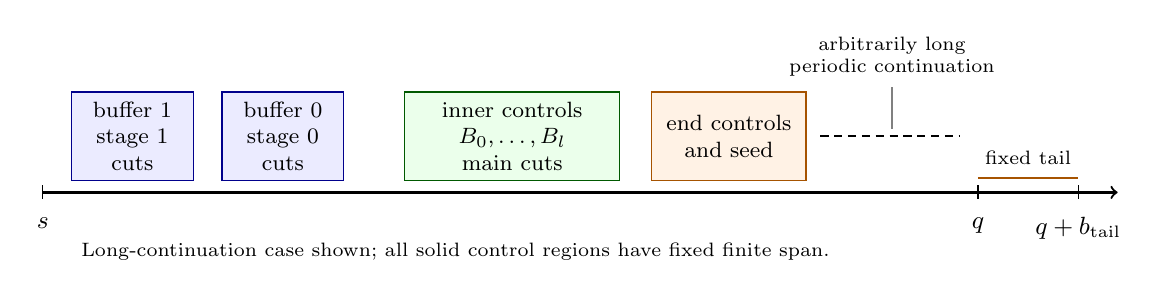
\begin{tikzpicture}[x=0.91cm,y=0.75cm,font=\small]
 \draw[->,thick] (0,0) -- (15,0);
 \draw (0,0.12) -- (0,-0.12) node[below=3pt] {$s$};
 \filldraw[fill=blue!8,draw=blue!55!black]
   (0.4,0.2) rectangle (2.1,1.7);
 \node[align=center,font=\footnotesize] at (1.25,0.95) {buffer $1$\\stage $1$\\cuts};
 \filldraw[fill=blue!8,draw=blue!55!black]
   (2.5,0.2) rectangle (4.2,1.7);
 \node[align=center,font=\footnotesize] at (3.35,0.95) {buffer $0$\\stage $0$\\cuts};
 \filldraw[fill=green!8,draw=green!35!black]
   (5.05,0.2) rectangle (8.05,1.7);
 \node[align=center,font=\footnotesize] at (6.55,0.95)
   {inner controls\\$B_0,\ldots,B_l$\\main cuts};
 \filldraw[fill=orange!10,draw=orange!65!black]
   (8.5,0.2) rectangle (10.65,1.7);
 \node[align=center,font=\footnotesize] at (9.575,0.95) {end controls\\and seed};
 \draw[densely dashed,thick] (10.85,0.95) -- (12.8,0.95);
 \draw[gray] (11.85,1.78) -- (11.85,1.08);
 \node[align=center,font=\scriptsize] at (11.85,2.3)
   {arbitrarily long\\periodic continuation};
 \draw (13.05,0.12) -- (13.05,-0.12)
   node[below=3pt] {$q$};
 \draw[thick,orange!65!black] (13.05,0.25) -- (14.45,0.25);
 \node[font=\scriptsize] at (13.75,0.58) {fixed tail};
 \draw (14.45,0.12) -- (14.45,-0.12)
   node[below=3pt,align=center] {$q+b_{\rm tail}$};
 \node[anchor=west,font=\scriptsize] at (0.4,-1.0)
   {Long-continuation case shown; all solid control regions have fixed finite span.};
\end{tikzpicture}

 \caption{The order of the computation regions in one episode, not to
 scale. A marker-absent episode with a long periodic continuation is shown.
 The control regions include bounded windows for translated hypotheses.
 With an earlier first mismatch, end-control windows may extend into the
 fixed tail; all remain before the episode endpoint $q+b_{\rm tail}$.}
 \label{fig:episode-schedule}
\end{figure}

\begin{definition}
Let $E$ consist of the nonempty words starting at $s$ for which the
required data are available, the anchor rule defines $q$, and the word
ends exactly at $q+b_{\rm tail}$.  The rule is interpreted using the
placement just fixed.  Since all tests translate with the letters, it
does not depend on an ambient coordinate origin.
\end{definition}

\begin{lemma}[Prefix code]
\label{lem:prefix-code}
The episode language $E$ is a prefix code: no member is a proper prefix
of another member.  All marker and bounded control decisions associated
with an episode are unchanged when letters are appended.
\end{lemma}

\begin{proof}
By Lemma~\ref{lem:placement}, each decision window is internal before
the prescribed endpoint.  Its letters therefore remain unchanged under
extension.  A present-marker anchor is unchanged.  In the absent case,
the seed and its periodic extension are unchanged, and the first mismatch
already seen remains the first mismatch.  Thus any extension has the same
prescribed endpoint.  It can be a complete episode only if it ends there.
\end{proof}

\subsection{A guard that forces the correct end}

An \emph{exact-end test at an origin} applies the anchor rule at that
origin and requires the entire test argument to end at
$q+b_{\rm tail}$.  In particular it includes the mismatch letter when
the marker is absent.  A suffix may make this test at a hypothesized
origin preceding its own start: it must still possess all the actual
seed and inspection windows required by that hypothesis.

For a fixed finite nonempty list of candidate origins, define its
\emph{end guard} to require equal values of $\eta$ at all candidates
and to apply the exact-end test at one fixed reference candidate.  The
list and reference are fixed by the suffix test's finite choices.  All
candidate windows are mandatory under the convention above.

\begin{lemma}[Exact end guard]
\label{lem:end-guard}
Suppose a finite word begins with a complete episode $e$ of true origin
$t$ and anchor $q$.  A prefix cut $k$ lies inside this first episode.
Let a suffix argument starting at $k$ use an end guard whose candidate
list contains $t$ and has diameter at most $w$.  If the guard accepts,
the suffix ends exactly at the end of $e$, and its reported anchor is
$q$.  This conclusion holds even if the proposed suffix initially ends
before $e$ or extends past $e$ into later letters.

On the actual suffix of $e$, the guard accepts whenever $A_1(t)$ is
false, provided the placement conditions for its list hold.
\end{lemma}

\begin{proof}
\emph{Agreement of the actual anchors.}
An accepted argument contains every mandatory window, so all the
candidate marker decisions agree with the corresponding decisions in the
containing word.  The true candidate therefore has its true value of
$\eta$.  If the common value is a present marker, the reference's
anchor is immediately $q$, and the exact-end test forces the claimed end.

Suppose instead that the common value is $\bot$.  Every candidate seed
has a period less than $d_e$.  Their starts differ by at most $w$, and
\[
 K_e-w>d_e^2.
\]
Their seeds consequently determine the same two-sided periodic word by
Lemma~\ref{lem:periodic-extension}.  The overlapping union of the seeds
consists entirely of letters of this word.  The true first mismatch is after the true seed. Every later candidate
seed starts before the true seed ends, since its displacement is at most
$w<K_e$. The mismatch cannot precede the start of such a seed, and it
cannot lie in any later candidate seed: that seed consists of actual letters of the same
periodic word, whereas the mismatch letter differs from it. A candidate
seed starting earlier also ends before the true seed ends. Thus the true
first mismatch follows the entire seed union.  It is therefore also the first mismatch after the reference
seed.

\emph{Rejection of premature and excessive consumption.}
For a proposed suffix ending too soon, either a mandatory window is
absent, or no earlier reference mismatch exists to certify its proposed
endpoint.  For a suffix extending too far, the actual first mismatch is
still the first one, so its exact-end test still requires the original
endpoint $q+b_{\rm tail}$.  Both cases are excluded.

\emph{Acceptance on a stable true episode.}
Finally, if $A_1(t)$ is false, every candidate is within distance $w$ of
$t$ and has the same $\eta$ value.  On the true suffix all windows are
available by placement.  The argument above shows that the reference
exact-end rule supplies the true endpoint, so the guard accepts.
\end{proof}

Only the reference candidate makes an unbounded continuation search in
this guard.  The other candidates supply bounded marker and seed data.
At the last residual stage we will instead decode the origin from bounded
data before making its one exact-end test.  These distinctions will also
be used to compile the suffix tests at height one.
